\documentclass[1p]{elsarticle_modified}
%\bibliographystyle{elsarticle-num}

%\usepackage[colorlinks]{hyperref}
%\usepackage{abbrmath_seonhwa} %\Abb, \Ascr, \Acal ,\Abf, \Afrak
\usepackage{amsfonts}
\usepackage{amssymb}
\usepackage{amsmath}
\usepackage{amsthm}
\usepackage{scalefnt}
\usepackage{amsbsy}
\usepackage{kotex}
\usepackage{caption}
\usepackage{subfig}
\usepackage{color}
\usepackage{graphicx}
\usepackage{xcolor} %% white, black, red, green, blue, cyan, magenta, yellow
\usepackage{float}
\usepackage{setspace}
\usepackage{hyperref}

\usepackage{tikz}
\usetikzlibrary{arrows}

\usepackage{multirow}
\usepackage{array} % fixed length table
\usepackage{hhline}

%%%%%%%%%%%%%%%%%%%%%
\makeatletter
\renewcommand*\env@matrix[1][\arraystretch]{%
	\edef\arraystretch{#1}%
	\hskip -\arraycolsep
	\let\@ifnextchar\new@ifnextchar
	\array{*\c@MaxMatrixCols c}}
\makeatother %https://tex.stackexchange.com/questions/14071/how-can-i-increase-the-line-spacing-in-a-matrix
%%%%%%%%%%%%%%%

\usepackage[normalem]{ulem}

\newcommand{\msout}[1]{\ifmmode\text{\sout{\ensuremath{#1}}}\else\sout{#1}\fi}
%SOURCE: \msout is \stkout macro in https://tex.stackexchange.com/questions/20609/strikeout-in-math-mode

\newcommand{\cancel}[1]{
	\ifmmode
	{\color{red}\msout{#1}}
	\else
	{\color{red}\sout{#1}}
	\fi
}

\newcommand{\add}[1]{
	{\color{blue}\uwave{#1}}
}

\newcommand{\replace}[2]{
	\ifmmode
	{\color{red}\msout{#1}}{\color{blue}\uwave{#2}}
	\else
	{\color{red}\sout{#1}}{\color{blue}\uwave{#2}}
	\fi
}

\newcommand{\Sol}{\mathcal{S}} %segment
\newcommand{\D}{D} %diagram
\newcommand{\A}{\mathcal{A}} %arc


%%%%%%%%%%%%%%%%%%%%%%%%%%%%%5 test

\def\sl{\operatorname{\textup{SL}}(2,\Cbb)}
\def\psl{\operatorname{\textup{PSL}}(2,\Cbb)}
\def\quan{\mkern 1mu \triangleright \mkern 1mu}

\theoremstyle{definition}
\newtheorem{thm}{Theorem}[section]
\newtheorem{prop}[thm]{Proposition}
\newtheorem{lem}[thm]{Lemma}
\newtheorem{ques}[thm]{Question}
\newtheorem{cor}[thm]{Corollary}
\newtheorem{defn}[thm]{Definition}
\newtheorem{exam}[thm]{Example}
\newtheorem{rmk}[thm]{Remark}
\newtheorem{alg}[thm]{Algorithm}

\newcommand{\I}{\sqrt{-1}}
\begin{document}

%\begin{frontmatter}
%
%\title{Boundary parabolic representations of knots up to 8 crossings}
%
%%% Group authors per affiliation:
%\author{Yunhi Cho} 
%\address{Department of Mathematics, University of Seoul, Seoul, Korea}
%\ead{yhcho@uos.ac.kr}
%
%
%\author{Seonhwa Kim} %\fnref{s_kim}}
%\address{Center for Geometry and Physics, Institute for Basic Science, Pohang, 37673, Korea}
%\ead{ryeona17@ibs.re.kr}
%
%\author{Hyuk Kim}
%\address{Department of Mathematical Sciences, Seoul National University, Seoul 08826, Korea}
%\ead{hyukkim@snu.ac.kr}
%
%\author{Seokbeom Yoon}
%\address{Department of Mathematical Sciences, Seoul National University, Seoul, 08826,  Korea}
%\ead{sbyoon15@snu.ac.kr}
%
%\begin{abstract}
%We find all boundary parabolic representation of knots up to 8 crossings.
%
%\end{abstract}
%\begin{keyword}
%    \MSC[2010] 57M25 
%\end{keyword}
%
%\end{frontmatter}

%\linenumbers
%\tableofcontents
%
\newcommand\colored[1]{\textcolor{white}{\rule[-0.35ex]{0.8em}{1.4ex}}\kern-0.8em\color{red} #1}%
%\newcommand\colored[1]{\textcolor{white}{ #1}\kern-2.17ex	\textcolor{white}{ #1}\kern-1.81ex	\textcolor{white}{ #1}\kern-2.15ex\color{red}#1	}

{\Large $\underline{12n_{0424}~(K12n_{0424})}$}

\setlength{\tabcolsep}{10pt}
\renewcommand{\arraystretch}{1.6}
\vspace{1cm}\begin{tabular}{m{100pt}>{\centering\arraybackslash}m{274pt}}
\multirow{5}{120pt}{
	\centering
	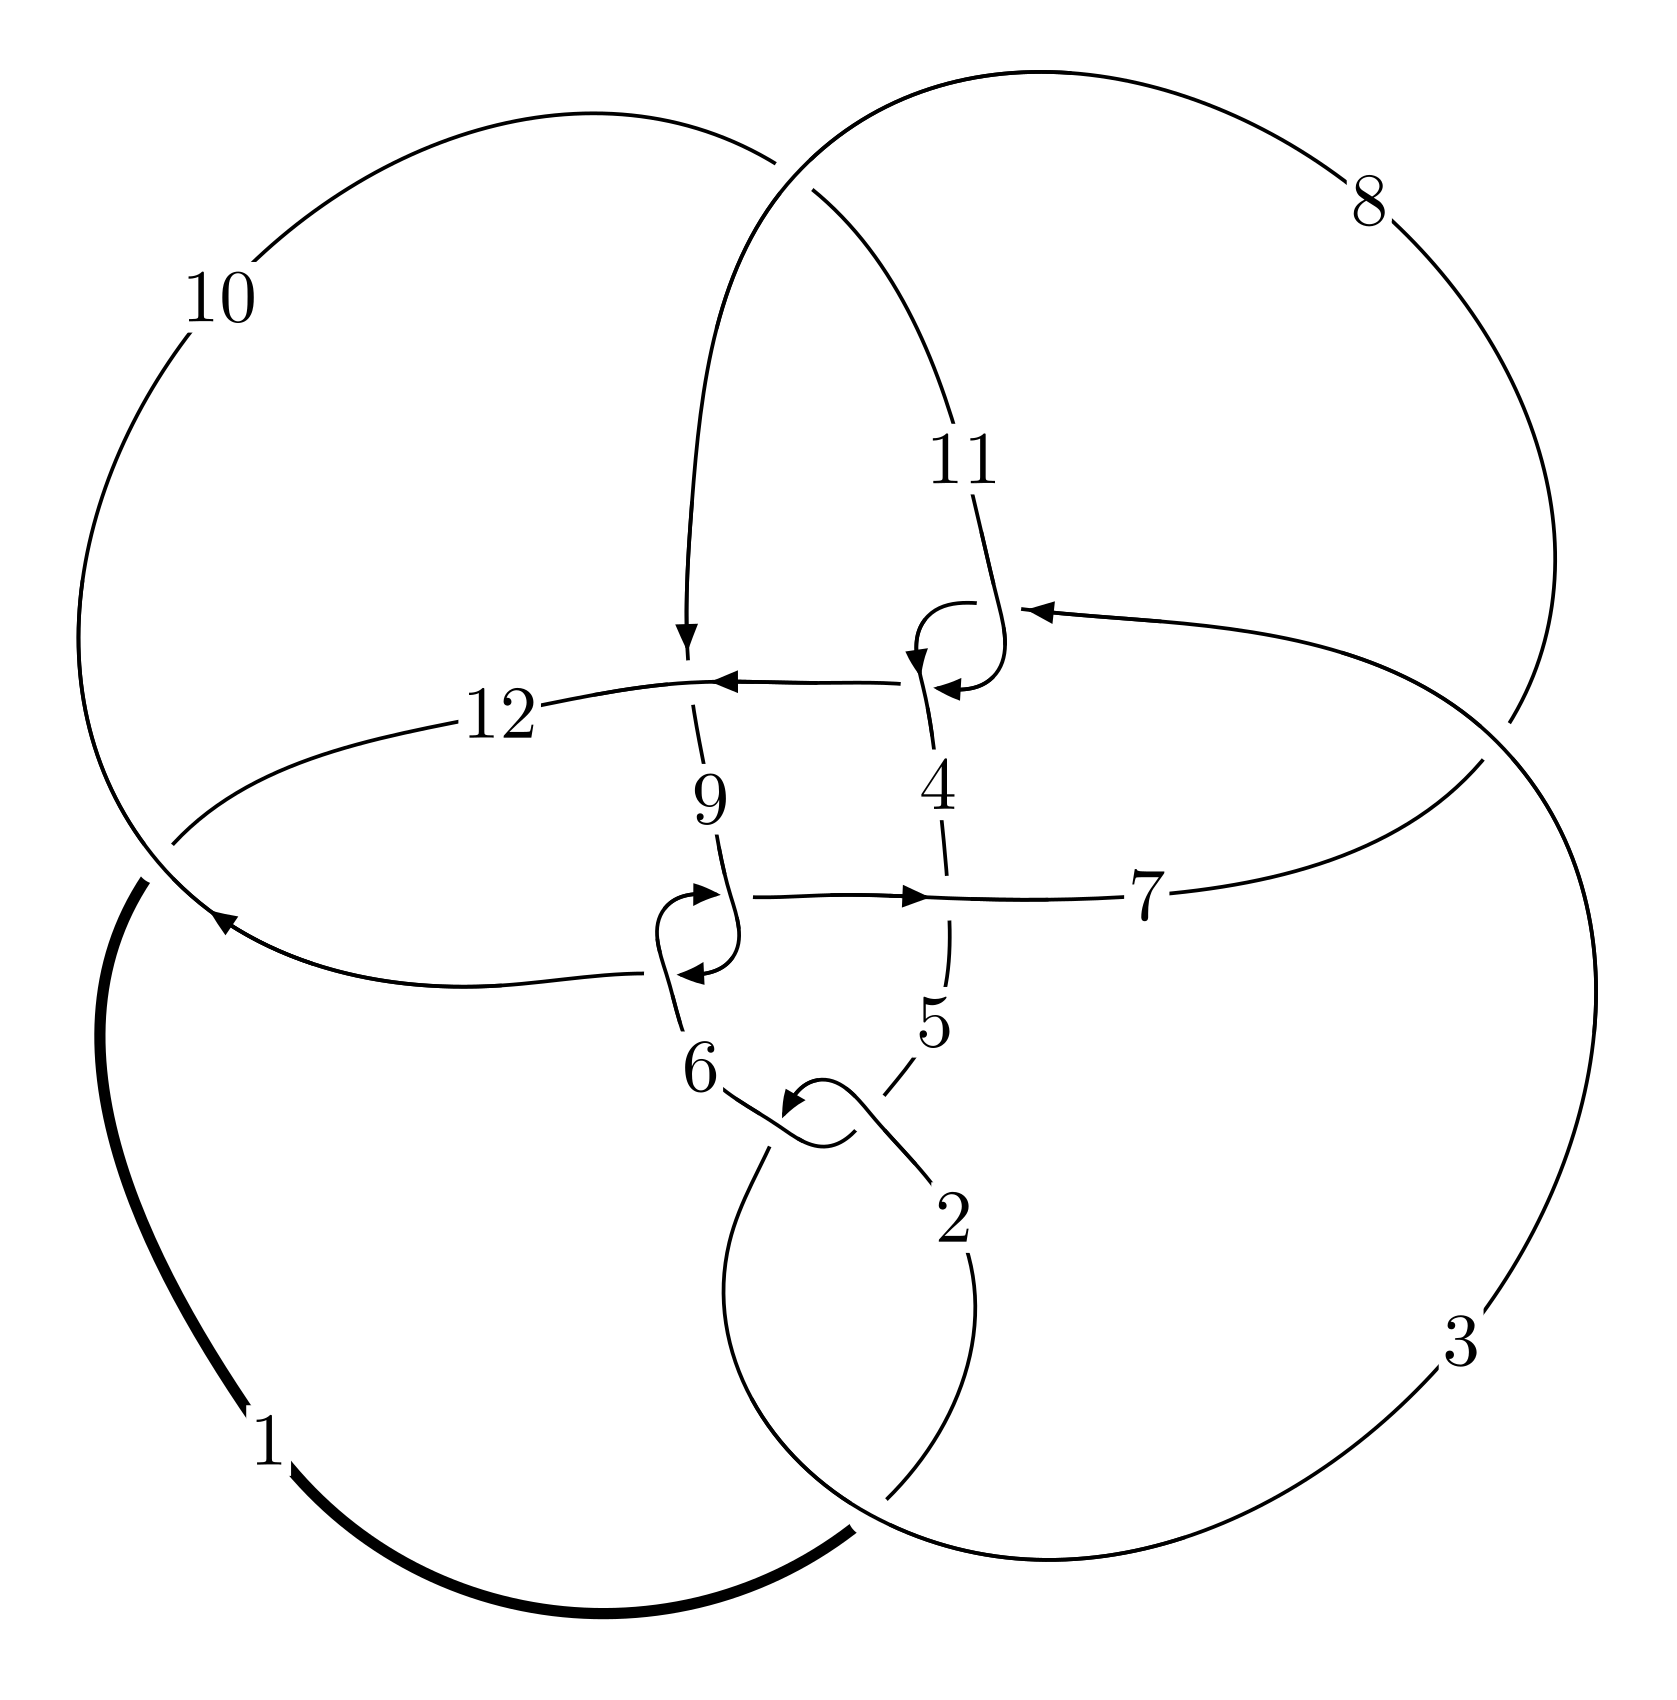
\includegraphics[width=112pt]{../../../GIT/diagram.site/Diagrams/png/2513_12n_0424.png}\\
\ \ \ A knot diagram\footnotemark}&
\allowdisplaybreaks
\textbf{Linearized knot diagam} \\
\cline{2-2}
 &
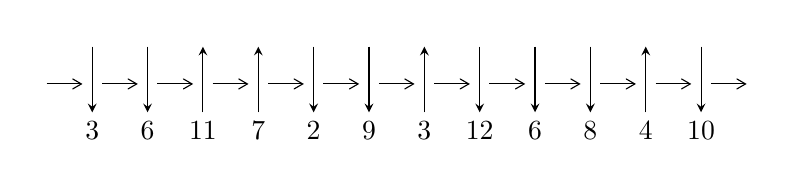
\begin{tikzpicture}[x=20pt, y=17pt]
	% nodes
	\node (C0) at (0, 0) {};
	\node (C1) at (1, 0) {};
	\node (C1U) at (1, +1) {};
	\node (C1D) at (1, -1) {3};

	\node (C2) at (2, 0) {};
	\node (C2U) at (2, +1) {};
	\node (C2D) at (2, -1) {6};

	\node (C3) at (3, 0) {};
	\node (C3U) at (3, +1) {};
	\node (C3D) at (3, -1) {11};

	\node (C4) at (4, 0) {};
	\node (C4U) at (4, +1) {};
	\node (C4D) at (4, -1) {7};

	\node (C5) at (5, 0) {};
	\node (C5U) at (5, +1) {};
	\node (C5D) at (5, -1) {2};

	\node (C6) at (6, 0) {};
	\node (C6U) at (6, +1) {};
	\node (C6D) at (6, -1) {9};

	\node (C7) at (7, 0) {};
	\node (C7U) at (7, +1) {};
	\node (C7D) at (7, -1) {3};

	\node (C8) at (8, 0) {};
	\node (C8U) at (8, +1) {};
	\node (C8D) at (8, -1) {12};

	\node (C9) at (9, 0) {};
	\node (C9U) at (9, +1) {};
	\node (C9D) at (9, -1) {6};

	\node (C10) at (10, 0) {};
	\node (C10U) at (10, +1) {};
	\node (C10D) at (10, -1) {8};

	\node (C11) at (11, 0) {};
	\node (C11U) at (11, +1) {};
	\node (C11D) at (11, -1) {4};

	\node (C12) at (12, 0) {};
	\node (C12U) at (12, +1) {};
	\node (C12D) at (12, -1) {10};
	\node (C13) at (13, 0) {};

	% arrows
	\draw[->,>={angle 60}]
	(C0) edge (C1) (C1) edge (C2) (C2) edge (C3) (C3) edge (C4) (C4) edge (C5) (C5) edge (C6) (C6) edge (C7) (C7) edge (C8) (C8) edge (C9) (C9) edge (C10) (C10) edge (C11) (C11) edge (C12) (C12) edge (C13) ;	\draw[->,>=stealth]
	(C1U) edge (C1D) (C2U) edge (C2D) (C3D) edge (C3U) (C4D) edge (C4U) (C5U) edge (C5D) (C6U) edge (C6D) (C7D) edge (C7U) (C8U) edge (C8D) (C9U) edge (C9D) (C10U) edge (C10D) (C11D) edge (C11U) (C12U) edge (C12D) ;
	\end{tikzpicture} \\
\hhline{~~} \\& 
\textbf{Solving Sequence} \\ \cline{2-2} 
 &
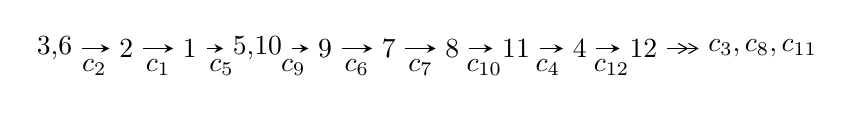
\begin{tikzpicture}[x=23pt, y=7pt]
	% node
	\node (A0) at (-1/8, 0) {3,6};
	\node (A1) at (1, 0) {2};
	\node (A2) at (2, 0) {1};
	\node (A3) at (49/16, 0) {5,10};
	\node (A4) at (33/8, 0) {9};
	\node (A5) at (41/8, 0) {7};
	\node (A6) at (49/8, 0) {8};
	\node (A7) at (57/8, 0) {11};
	\node (A8) at (65/8, 0) {4};
	\node (A9) at (73/8, 0) {12};
	\node (C1) at (1/2, -1) {$c_{2}$};
	\node (C2) at (3/2, -1) {$c_{1}$};
	\node (C3) at (5/2, -1) {$c_{5}$};
	\node (C4) at (29/8, -1) {$c_{9}$};
	\node (C5) at (37/8, -1) {$c_{6}$};
	\node (C6) at (45/8, -1) {$c_{7}$};
	\node (C7) at (53/8, -1) {$c_{10}$};
	\node (C8) at (61/8, -1) {$c_{4}$};
	\node (C9) at (69/8, -1) {$c_{12}$};
	\node (A10) at (11, 0) {$c_{3},c_{8},c_{11}$};

	% edge
	\draw[->,>=stealth]	
	(A0) edge (A1) (A1) edge (A2) (A2) edge (A3) (A3) edge (A4) (A4) edge (A5) (A5) edge (A6) (A6) edge (A7) (A7) edge (A8) (A8) edge (A9) ;
	\draw[->>,>={angle 60}]	
	(A9) edge (A10);
\end{tikzpicture} \\ 

\end{tabular} \\

\footnotetext{
The image of knot diagram is generated by the software ``\textbf{Draw programme}" developed by Andrew Bartholomew(\url{http://www.layer8.co.uk/maths/draw/index.htm\#Running-draw}), where we modified some parts for our purpose(\url{https://github.com/CATsTAILs/LinksPainter}).
}\phantom \\ \newline 
\centering \textbf{Ideals for irreducible components\footnotemark of $X_{\text{par}}$} 
 
\begin{align*}
I^u_{1}&=\langle 
2.60349\times10^{202} u^{67}-1.26475\times10^{203} u^{66}+\cdots+3.63435\times10^{205} b+1.56735\times10^{205},\\
\phantom{I^u_{1}}&\phantom{= \langle  }2.69439\times10^{205} u^{67}-1.16805\times10^{206} u^{66}+\cdots+1.15209\times10^{208} a+8.44586\times10^{207},\\
\phantom{I^u_{1}}&\phantom{= \langle  }u^{68}-5 u^{67}+\cdots+86 u-317\rangle \\
I^u_{2}&=\langle 
56939 u^{20}+161982 u^{19}+\cdots+59123 b+87648,\;299698 u^{20}+645903 u^{19}+\cdots+59123 a+588498,\\
\phantom{I^u_{2}}&\phantom{= \langle  }u^{21}+2 u^{20}+\cdots+4 u-1\rangle \\
\\
\end{align*}
\raggedright * 2 irreducible components of $\dim_{\mathbb{C}}=0$, with total 89 representations.\\
\footnotetext{All coefficients of polynomials are rational numbers. But the coefficients are sometimes approximated in decimal forms when there is not enough margin.}
\newpage
\renewcommand{\arraystretch}{1}
\centering \section*{I. $I^u_{1}= \langle 2.60\times10^{202} u^{67}-1.26\times10^{203} u^{66}+\cdots+3.63\times10^{205} b+1.57\times10^{205},\;2.69\times10^{205} u^{67}-1.17\times10^{206} u^{66}+\cdots+1.15\times10^{208} a+8.45\times10^{207},\;u^{68}-5 u^{67}+\cdots+86 u-317 \rangle$}
\flushleft \textbf{(i) Arc colorings}\\
\begin{tabular}{m{7pt} m{180pt} m{7pt} m{180pt} }
\flushright $a_{3}=$&$\begin{pmatrix}1\\0\end{pmatrix}$ \\
\flushright $a_{6}=$&$\begin{pmatrix}0\\u\end{pmatrix}$ \\
\flushright $a_{2}=$&$\begin{pmatrix}1\\- u^2\end{pmatrix}$ \\
\flushright $a_{1}=$&$\begin{pmatrix}- u^2+1\\- u^2\end{pmatrix}$ \\
\flushright $a_{5}=$&$\begin{pmatrix}u\\- u^3+u\end{pmatrix}$ \\
\flushright $a_{10}=$&$\begin{pmatrix}-0.00233870 u^{67}+0.0101386 u^{66}+\cdots-11.2417 u-0.733090\\-0.000716356 u^{67}+0.00347999 u^{66}+\cdots-5.24442 u-0.431259\end{pmatrix}$ \\
\flushright $a_{9}=$&$\begin{pmatrix}-0.00233870 u^{67}+0.0101386 u^{66}+\cdots-11.2417 u-0.733090\\-0.00117955 u^{67}+0.00620829 u^{66}+\cdots-4.63678 u+0.0616603\end{pmatrix}$ \\
\flushright $a_{7}=$&$\begin{pmatrix}0.00491528 u^{67}-0.0262227 u^{66}+\cdots+25.2225 u+6.20953\\-0.000952899 u^{67}+0.00487972 u^{66}+\cdots+0.0569866 u+0.671964\end{pmatrix}$ \\
\flushright $a_{8}=$&$\begin{pmatrix}0.00396238 u^{67}-0.0213429 u^{66}+\cdots+25.2795 u+6.88149\\-0.000952899 u^{67}+0.00487972 u^{66}+\cdots+0.0569866 u+0.671964\end{pmatrix}$ \\
\flushright $a_{11}=$&$\begin{pmatrix}0.00373541 u^{67}-0.0186514 u^{66}+\cdots+30.2287 u+11.1920\\-0.000136580 u^{67}+0.000781749 u^{66}+\cdots+3.37713 u+0.340186\end{pmatrix}$ \\
\flushright $a_{4}=$&$\begin{pmatrix}-0.00276461 u^{67}+0.0125786 u^{66}+\cdots-47.0972 u-12.3994\\-0.0000159099 u^{67}+0.000183427 u^{66}+\cdots-4.26921 u+0.0576805\end{pmatrix}$ \\
\flushright $a_{12}=$&$\begin{pmatrix}-0.000531157 u^{67}+0.00366050 u^{66}+\cdots+31.7108 u+3.30930\\-0.00101402 u^{67}+0.00536595 u^{66}+\cdots+0.703120 u-0.416678\end{pmatrix}$\\&\end{tabular}
\flushleft \textbf{(ii) Obstruction class $= -1$}\\~\\
\flushleft \textbf{(iii) Cusp Shapes $= -0.00431587 u^{67}+0.0232128 u^{66}+\cdots+33.1103 u+8.26277$}\\~\\
\newpage\renewcommand{\arraystretch}{1}
\flushleft \textbf{(iv) u-Polynomials at the component}\newline \\
\begin{tabular}{m{50pt}|m{274pt}}
Crossings & \hspace{64pt}u-Polynomials at each crossing \\
\hline $$\begin{aligned}c_{1}\end{aligned}$$&$\begin{aligned}
&u^{68}+81 u^{67}+\cdots+7054940 u+100489
\end{aligned}$\\
\hline $$\begin{aligned}c_{2},c_{5}\end{aligned}$$&$\begin{aligned}
&u^{68}+5 u^{67}+\cdots-86 u-317
\end{aligned}$\\
\hline $$\begin{aligned}c_{3},c_{11}\end{aligned}$$&$\begin{aligned}
&u^{68}-23 u^{66}+\cdots+2 u+1
\end{aligned}$\\
\hline $$\begin{aligned}c_{4}\end{aligned}$$&$\begin{aligned}
&u^{68}+12 u^{67}+\cdots-352006 u+2124268
\end{aligned}$\\
\hline $$\begin{aligned}c_{6},c_{9}\end{aligned}$$&$\begin{aligned}
&u^{68}+6 u^{67}+\cdots-23 u+1
\end{aligned}$\\
\hline $$\begin{aligned}c_{7}\end{aligned}$$&$\begin{aligned}
&u^{68}-3 u^{67}+\cdots+4608 u-512
\end{aligned}$\\
\hline $$\begin{aligned}c_{8}\end{aligned}$$&$\begin{aligned}
&u^{68}+u^{67}+\cdots+30 u-4
\end{aligned}$\\
\hline $$\begin{aligned}c_{10}\end{aligned}$$&$\begin{aligned}
&u^{68}+4 u^{65}+\cdots+101 u+41
\end{aligned}$\\
\hline $$\begin{aligned}c_{12}\end{aligned}$$&$\begin{aligned}
&u^{68}-15 u^{67}+\cdots+4125551 u-99557
\end{aligned}$\\
\hline
\end{tabular}\\~\\
\newpage\renewcommand{\arraystretch}{1}
\flushleft \textbf{(v) Riley Polynomials at the component}\newline \\
\begin{tabular}{m{50pt}|m{274pt}}
Crossings & \hspace{64pt}Riley Polynomials at each crossing \\
\hline $$\begin{aligned}c_{1}\end{aligned}$$&$\begin{aligned}
&y^{68}-173 y^{67}+\cdots+1338138438004 y+10098039121
\end{aligned}$\\
\hline $$\begin{aligned}c_{2},c_{5}\end{aligned}$$&$\begin{aligned}
&y^{68}-81 y^{67}+\cdots-7054940 y+100489
\end{aligned}$\\
\hline $$\begin{aligned}c_{3},c_{11}\end{aligned}$$&$\begin{aligned}
&y^{68}-46 y^{67}+\cdots+10 y+1
\end{aligned}$\\
\hline $$\begin{aligned}c_{4}\end{aligned}$$&$\begin{aligned}
&y^{68}+72 y^{67}+\cdots+70533073386900 y+4512514535824
\end{aligned}$\\
\hline $$\begin{aligned}c_{6},c_{9}\end{aligned}$$&$\begin{aligned}
&y^{68}+12 y^{67}+\cdots-193 y+1
\end{aligned}$\\
\hline $$\begin{aligned}c_{7}\end{aligned}$$&$\begin{aligned}
&y^{68}+21 y^{67}+\cdots+15597568 y+262144
\end{aligned}$\\
\hline $$\begin{aligned}c_{8}\end{aligned}$$&$\begin{aligned}
&y^{68}-3 y^{67}+\cdots+100 y+16
\end{aligned}$\\
\hline $$\begin{aligned}c_{10}\end{aligned}$$&$\begin{aligned}
&y^{68}+60 y^{66}+\cdots-19877 y+1681
\end{aligned}$\\
\hline $$\begin{aligned}c_{12}\end{aligned}$$&$\begin{aligned}
&y^{68}-59 y^{67}+\cdots-745245389293 y+9911596249
\end{aligned}$\\
\hline
\end{tabular}\\~\\
\newpage\flushleft \textbf{(vi) Complex Volumes and Cusp Shapes}
$$\begin{array}{c|c|c}  
\text{Solutions to }I^u_{1}& \I (\text{vol} + \sqrt{-1}CS) & \text{Cusp shape}\\
 \hline 
\begin{aligned}
u &= \phantom{-}0.871128 + 0.509881 I \\
a &= -0.251428 - 0.802924 I \\
b &= \phantom{-}0.018453 + 0.953747 I\end{aligned}
 & -1.05916 - 0.94846 I & \phantom{-0.000000 } 0 \\ \hline\begin{aligned}
u &= \phantom{-}0.871128 - 0.509881 I \\
a &= -0.251428 + 0.802924 I \\
b &= \phantom{-}0.018453 - 0.953747 I\end{aligned}
 & -1.05916 + 0.94846 I & \phantom{-0.000000 } 0 \\ \hline\begin{aligned}
u &= -0.544948 + 0.820477 I \\
a &= -0.774935 + 0.270468 I \\
b &= -1.058330 + 0.233379 I\end{aligned}
 & \phantom{-}4.15929 - 0.82146 I & \phantom{-0.000000 } 0 \\ \hline\begin{aligned}
u &= -0.544948 - 0.820477 I \\
a &= -0.774935 - 0.270468 I \\
b &= -1.058330 - 0.233379 I\end{aligned}
 & \phantom{-}4.15929 + 0.82146 I & \phantom{-0.000000 } 0 \\ \hline\begin{aligned}
u &= \phantom{-}1.046280 + 0.158379 I \\
a &= -0.05036 + 1.45147 I \\
b &= \phantom{-}0.389019 + 0.679852 I\end{aligned}
 & \phantom{-}4.06606 + 4.41418 I & \phantom{-0.000000 } 0 \\ \hline\begin{aligned}
u &= \phantom{-}1.046280 - 0.158379 I \\
a &= -0.05036 - 1.45147 I \\
b &= \phantom{-}0.389019 - 0.679852 I\end{aligned}
 & \phantom{-}4.06606 - 4.41418 I & \phantom{-0.000000 } 0 \\ \hline\begin{aligned}
u &= -0.885188 + 0.133345 I \\
a &= -0.609940 + 0.064726 I \\
b &= -0.36252 + 1.60437 I\end{aligned}
 & \phantom{-}2.00126 + 7.10030 I & -5.49116 - 6.13012 I \\ \hline\begin{aligned}
u &= -0.885188 - 0.133345 I \\
a &= -0.609940 - 0.064726 I \\
b &= -0.36252 - 1.60437 I\end{aligned}
 & \phantom{-}2.00126 - 7.10030 I & -5.49116 + 6.13012 I \\ \hline\begin{aligned}
u &= \phantom{-}0.440543 + 0.709904 I \\
a &= -0.925199 + 0.715716 I \\
b &= -0.563366 + 0.659728 I\end{aligned}
 & -0.315752 - 0.651012 I & -5.42332 - 3.40225 I \\ \hline\begin{aligned}
u &= \phantom{-}0.440543 - 0.709904 I \\
a &= -0.925199 - 0.715716 I \\
b &= -0.563366 - 0.659728 I\end{aligned}
 & -0.315752 + 0.651012 I & -5.42332 + 3.40225 I\\
 \hline 
 \end{array}$$\newpage$$\begin{array}{c|c|c}  
\text{Solutions to }I^u_{1}& \I (\text{vol} + \sqrt{-1}CS) & \text{Cusp shape}\\
 \hline 
\begin{aligned}
u &= \phantom{-}0.800978 + 0.142572 I \\
a &= \phantom{-}0.366163 - 0.014633 I \\
b &= \phantom{-}0.69817 + 1.28569 I\end{aligned}
 & -1.37004 - 1.79460 I & -8.18525 + 5.97883 I \\ \hline\begin{aligned}
u &= \phantom{-}0.800978 - 0.142572 I \\
a &= \phantom{-}0.366163 + 0.014633 I \\
b &= \phantom{-}0.69817 - 1.28569 I\end{aligned}
 & -1.37004 + 1.79460 I & -8.18525 - 5.97883 I \\ \hline\begin{aligned}
u &= -0.188648 + 0.784530 I \\
a &= \phantom{-}1.113550 + 0.741221 I \\
b &= \phantom{-}0.823409 + 0.516607 I\end{aligned}
 & \phantom{-}0.44809 + 2.22556 I & -2.79693 - 5.37400 I \\ \hline\begin{aligned}
u &= -0.188648 - 0.784530 I \\
a &= \phantom{-}1.113550 - 0.741221 I \\
b &= \phantom{-}0.823409 - 0.516607 I\end{aligned}
 & \phantom{-}0.44809 - 2.22556 I & -2.79693 + 5.37400 I \\ \hline\begin{aligned}
u &= -1.042970 + 0.640059 I \\
a &= \phantom{-}0.252793 - 0.689948 I \\
b &= \phantom{-}0.583572 + 0.375949 I\end{aligned}
 & \phantom{-}2.60331 + 6.17342 I & \phantom{-0.000000 } 0 \\ \hline\begin{aligned}
u &= -1.042970 - 0.640059 I \\
a &= \phantom{-}0.252793 + 0.689948 I \\
b &= \phantom{-}0.583572 - 0.375949 I\end{aligned}
 & \phantom{-}2.60331 - 6.17342 I & \phantom{-0.000000 } 0 \\ \hline\begin{aligned}
u &= -0.588960 + 0.496925 I \\
a &= -0.393461 + 1.028770 I \\
b &= \phantom{-}0.135056 + 0.879028 I\end{aligned}
 & \phantom{-}1.71068 - 2.22744 I & -2.20317 + 3.51892 I \\ \hline\begin{aligned}
u &= -0.588960 - 0.496925 I \\
a &= -0.393461 - 1.028770 I \\
b &= \phantom{-}0.135056 - 0.879028 I\end{aligned}
 & \phantom{-}1.71068 + 2.22744 I & -2.20317 - 3.51892 I \\ \hline\begin{aligned}
u &= \phantom{-}0.558593 + 0.526304 I \\
a &= -0.860916 - 0.104097 I \\
b &= -0.292526 + 0.378622 I\end{aligned}
 & -0.41361 - 1.51672 I & -4.11702 + 3.50590 I \\ \hline\begin{aligned}
u &= \phantom{-}0.558593 - 0.526304 I \\
a &= -0.860916 + 0.104097 I \\
b &= -0.292526 - 0.378622 I\end{aligned}
 & -0.41361 + 1.51672 I & -4.11702 - 3.50590 I\\
 \hline 
 \end{array}$$\newpage$$\begin{array}{c|c|c}  
\text{Solutions to }I^u_{1}& \I (\text{vol} + \sqrt{-1}CS) & \text{Cusp shape}\\
 \hline 
\begin{aligned}
u &= -0.698428 + 0.225559 I \\
a &= -0.06120 + 1.66744 I \\
b &= \phantom{-}0.059794 + 0.692238 I\end{aligned}
 & \phantom{-}1.94783 - 2.44722 I & \phantom{-}0.47230 - 2.86417 I \\ \hline\begin{aligned}
u &= -0.698428 - 0.225559 I \\
a &= -0.06120 - 1.66744 I \\
b &= \phantom{-}0.059794 - 0.692238 I\end{aligned}
 & \phantom{-}1.94783 + 2.44722 I & \phantom{-}0.47230 + 2.86417 I \\ \hline\begin{aligned}
u &= -1.149490 + 0.645257 I \\
a &= -0.244780 + 0.273572 I \\
b &= \phantom{-}0.201289 + 0.916767 I\end{aligned}
 & \phantom{-}2.21731 - 2.65488 I & \phantom{-0.000000 } 0 \\ \hline\begin{aligned}
u &= -1.149490 - 0.645257 I \\
a &= -0.244780 - 0.273572 I \\
b &= \phantom{-}0.201289 - 0.916767 I\end{aligned}
 & \phantom{-}2.21731 + 2.65488 I & \phantom{-0.000000 } 0 \\ \hline\begin{aligned}
u &= -0.734034 + 1.108720 I \\
a &= -0.095793 - 0.323746 I \\
b &= -0.023606 + 0.235560 I\end{aligned}
 & \phantom{-}1.83474 - 2.80065 I & \phantom{-0.000000 } 0 \\ \hline\begin{aligned}
u &= -0.734034 - 1.108720 I \\
a &= -0.095793 + 0.323746 I \\
b &= -0.023606 - 0.235560 I\end{aligned}
 & \phantom{-}1.83474 + 2.80065 I & \phantom{-0.000000 } 0 \\ \hline\begin{aligned}
u &= -0.537572 + 0.292817 I \\
a &= \phantom{-}1.59768 - 1.26454 I \\
b &= \phantom{-}0.424708 - 0.016900 I\end{aligned}
 & \phantom{-}1.85960 + 4.70737 I & -2.52304 - 10.70995 I \\ \hline\begin{aligned}
u &= -0.537572 - 0.292817 I \\
a &= \phantom{-}1.59768 + 1.26454 I \\
b &= \phantom{-}0.424708 + 0.016900 I\end{aligned}
 & \phantom{-}1.85960 - 4.70737 I & -2.52304 + 10.70995 I \\ \hline\begin{aligned}
u &= -0.753527 + 1.166220 I \\
a &= -0.762293 - 0.164274 I \\
b &= -0.822320 + 0.177075 I\end{aligned}
 & \phantom{-}1.79765 + 10.38310 I & \phantom{-0.000000 } 0 \\ \hline\begin{aligned}
u &= -0.753527 - 1.166220 I \\
a &= -0.762293 + 0.164274 I \\
b &= -0.822320 - 0.177075 I\end{aligned}
 & \phantom{-}1.79765 - 10.38310 I & \phantom{-0.000000 } 0\\
 \hline 
 \end{array}$$\newpage$$\begin{array}{c|c|c}  
\text{Solutions to }I^u_{1}& \I (\text{vol} + \sqrt{-1}CS) & \text{Cusp shape}\\
 \hline 
\begin{aligned}
u &= \phantom{-}0.474569 + 0.362132 I \\
a &= -1.72365 + 0.23562 I \\
b &= -0.443265 + 0.309260 I\end{aligned}
 & -0.87147 - 2.49560 I & -8.19061 + 9.19024 I \\ \hline\begin{aligned}
u &= \phantom{-}0.474569 - 0.362132 I \\
a &= -1.72365 - 0.23562 I \\
b &= -0.443265 - 0.309260 I\end{aligned}
 & -0.87147 + 2.49560 I & -8.19061 - 9.19024 I \\ \hline\begin{aligned}
u &= \phantom{-}0.830722 + 1.137770 I \\
a &= \phantom{-}0.613745 - 0.111412 I \\
b &= \phantom{-}0.732990 + 0.363720 I\end{aligned}
 & -2.05341 - 4.26526 I & \phantom{-0.000000 } 0 \\ \hline\begin{aligned}
u &= \phantom{-}0.830722 - 1.137770 I \\
a &= \phantom{-}0.613745 + 0.111412 I \\
b &= \phantom{-}0.732990 - 0.363720 I\end{aligned}
 & -2.05341 + 4.26526 I & \phantom{-0.000000 } 0 \\ \hline\begin{aligned}
u &= -0.429455 + 0.392611 I \\
a &= \phantom{-}0.56873 - 1.67827 I \\
b &= -0.460162 + 1.313910 I\end{aligned}
 & \phantom{-}3.56883 - 5.49597 I & -0.35708 + 7.00581 I \\ \hline\begin{aligned}
u &= -0.429455 - 0.392611 I \\
a &= \phantom{-}0.56873 + 1.67827 I \\
b &= -0.460162 - 1.313910 I\end{aligned}
 & \phantom{-}3.56883 + 5.49597 I & -0.35708 - 7.00581 I \\ \hline\begin{aligned}
u &= -1.43036\phantom{ +0.000000I} \\
a &= -0.0534743\phantom{ +0.000000I} \\
b &= -1.45724\phantom{ +0.000000I}\end{aligned}
 & -3.29592\phantom{ +0.000000I} & \phantom{-0.000000 } 0 \\ \hline\begin{aligned}
u &= \phantom{-}1.45239 + 0.17220 I \\
a &= -0.751230 - 0.429370 I \\
b &= -2.36893 - 0.07099 I\end{aligned}
 & -6.96130 - 1.46154 I & \phantom{-0.000000 } 0 \\ \hline\begin{aligned}
u &= \phantom{-}1.45239 - 0.17220 I \\
a &= -0.751230 + 0.429370 I \\
b &= -2.36893 + 0.07099 I\end{aligned}
 & -6.96130 + 1.46154 I & \phantom{-0.000000 } 0 \\ \hline\begin{aligned}
u &= \phantom{-}1.46944\phantom{ +0.000000I} \\
a &= \phantom{-}0.392688\phantom{ +0.000000I} \\
b &= \phantom{-}1.69276\phantom{ +0.000000I}\end{aligned}
 & -3.78770\phantom{ +0.000000I} & \phantom{-0.000000 } 0\\
 \hline 
 \end{array}$$\newpage$$\begin{array}{c|c|c}  
\text{Solutions to }I^u_{1}& \I (\text{vol} + \sqrt{-1}CS) & \text{Cusp shape}\\
 \hline 
\begin{aligned}
u &= -1.55873 + 0.13384 I \\
a &= \phantom{-}0.852639 - 0.619616 I \\
b &= \phantom{-}2.29095 - 0.57702 I\end{aligned}
 & -7.71397 + 4.42312 I & \phantom{-0.000000 } 0 \\ \hline\begin{aligned}
u &= -1.55873 - 0.13384 I \\
a &= \phantom{-}0.852639 + 0.619616 I \\
b &= \phantom{-}2.29095 + 0.57702 I\end{aligned}
 & -7.71397 - 4.42312 I & \phantom{-0.000000 } 0 \\ \hline\begin{aligned}
u &= \phantom{-}1.58955 + 0.06373 I \\
a &= -0.636720 - 0.744311 I \\
b &= -1.89607 - 0.94307 I\end{aligned}
 & -5.50713 - 5.89389 I & \phantom{-0.000000 } 0 \\ \hline\begin{aligned}
u &= \phantom{-}1.58955 - 0.06373 I \\
a &= -0.636720 + 0.744311 I \\
b &= -1.89607 + 0.94307 I\end{aligned}
 & -5.50713 + 5.89389 I & \phantom{-0.000000 } 0 \\ \hline\begin{aligned}
u &= -1.63011 + 0.19482 I \\
a &= \phantom{-}0.777479 - 0.591084 I \\
b &= \phantom{-}1.98605 - 0.45195 I\end{aligned}
 & -8.12749 + 4.22844 I & \phantom{-0.000000 } 0 \\ \hline\begin{aligned}
u &= -1.63011 - 0.19482 I \\
a &= \phantom{-}0.777479 + 0.591084 I \\
b &= \phantom{-}1.98605 + 0.45195 I\end{aligned}
 & -8.12749 - 4.22844 I & \phantom{-0.000000 } 0 \\ \hline\begin{aligned}
u &= \phantom{-}1.60712 + 0.36324 I \\
a &= -0.745239 - 0.676686 I \\
b &= -1.82570 - 0.29640 I\end{aligned}
 & -5.64912 - 6.82670 I & \phantom{-0.000000 } 0 \\ \hline\begin{aligned}
u &= \phantom{-}1.60712 - 0.36324 I \\
a &= -0.745239 + 0.676686 I \\
b &= -1.82570 + 0.29640 I\end{aligned}
 & -5.64912 + 6.82670 I & \phantom{-0.000000 } 0 \\ \hline\begin{aligned}
u &= -0.297585 + 0.072176 I \\
a &= \phantom{-}2.48257 + 0.33875 I \\
b &= \phantom{-}0.492290 + 0.055394 I\end{aligned}
 & -1.42607 + 0.01276 I & -9.44279 + 0.81659 I \\ \hline\begin{aligned}
u &= -0.297585 - 0.072176 I \\
a &= \phantom{-}2.48257 - 0.33875 I \\
b &= \phantom{-}0.492290 - 0.055394 I\end{aligned}
 & -1.42607 - 0.01276 I & -9.44279 - 0.81659 I\\
 \hline 
 \end{array}$$\newpage$$\begin{array}{c|c|c}  
\text{Solutions to }I^u_{1}& \I (\text{vol} + \sqrt{-1}CS) & \text{Cusp shape}\\
 \hline 
\begin{aligned}
u &= -1.70975 + 0.05552 I \\
a &= -0.624502 - 0.582986 I \\
b &= -1.88329 - 0.29548 I\end{aligned}
 & -10.76850 + 2.56396 I & \phantom{-0.000000 } 0 \\ \hline\begin{aligned}
u &= -1.70975 - 0.05552 I \\
a &= -0.624502 + 0.582986 I \\
b &= -1.88329 + 0.29548 I\end{aligned}
 & -10.76850 - 2.56396 I & \phantom{-0.000000 } 0 \\ \hline\begin{aligned}
u &= \phantom{-}1.71065 + 0.07105 I \\
a &= \phantom{-}0.732714 - 0.538117 I \\
b &= \phantom{-}1.95223 - 0.29659 I\end{aligned}
 & -7.52248 - 8.09991 I & \phantom{-0.000000 } 0 \\ \hline\begin{aligned}
u &= \phantom{-}1.71065 - 0.07105 I \\
a &= \phantom{-}0.732714 + 0.538117 I \\
b &= \phantom{-}1.95223 + 0.29659 I\end{aligned}
 & -7.52248 + 8.09991 I & \phantom{-0.000000 } 0 \\ \hline\begin{aligned}
u &= -1.74721 + 0.17347 I \\
a &= \phantom{-}0.813534 - 0.514883 I \\
b &= \phantom{-}1.85421 - 0.43442 I\end{aligned}
 & -8.31422 + 4.53840 I & \phantom{-0.000000 } 0 \\ \hline\begin{aligned}
u &= -1.74721 - 0.17347 I \\
a &= \phantom{-}0.813534 + 0.514883 I \\
b &= \phantom{-}1.85421 + 0.43442 I\end{aligned}
 & -8.31422 - 4.53840 I & \phantom{-0.000000 } 0 \\ \hline\begin{aligned}
u &= \phantom{-}1.72573 + 0.38376 I \\
a &= \phantom{-}0.702168 + 0.550948 I \\
b &= \phantom{-}2.08835 + 0.55587 I\end{aligned}
 & -6.2957 - 16.2757 I & \phantom{-0.000000 } 0 \\ \hline\begin{aligned}
u &= \phantom{-}1.72573 - 0.38376 I \\
a &= \phantom{-}0.702168 - 0.550948 I \\
b &= \phantom{-}2.08835 - 0.55587 I\end{aligned}
 & -6.2957 + 16.2757 I & \phantom{-0.000000 } 0 \\ \hline\begin{aligned}
u &= -1.73754 + 0.38845 I \\
a &= -0.676834 + 0.471111 I \\
b &= -2.07579 + 0.51144 I\end{aligned}
 & -10.3272 + 10.1790 I & \phantom{-0.000000 } 0 \\ \hline\begin{aligned}
u &= -1.73754 - 0.38845 I \\
a &= -0.676834 - 0.471111 I \\
b &= -2.07579 - 0.51144 I\end{aligned}
 & -10.3272 - 10.1790 I & \phantom{-0.000000 } 0\\
 \hline 
 \end{array}$$\newpage$$\begin{array}{c|c|c}  
\text{Solutions to }I^u_{1}& \I (\text{vol} + \sqrt{-1}CS) & \text{Cusp shape}\\
 \hline 
\begin{aligned}
u &= \phantom{-}0.186071 + 0.088469 I \\
a &= \phantom{-}2.84558 + 5.76663 I \\
b &= -0.584481 + 0.792155 I\end{aligned}
 & \phantom{-}6.79008 + 4.75733 I & \phantom{-}3.79704 - 5.76566 I \\ \hline\begin{aligned}
u &= \phantom{-}0.186071 - 0.088469 I \\
a &= \phantom{-}2.84558 - 5.76663 I \\
b &= -0.584481 - 0.792155 I\end{aligned}
 & \phantom{-}6.79008 - 4.75733 I & \phantom{-}3.79704 + 5.76566 I \\ \hline\begin{aligned}
u &= \phantom{-}1.79378 + 0.03621 I \\
a &= -0.667026 - 0.311610 I \\
b &= -1.61634 - 0.35448 I\end{aligned}
 & -8.03735 - 1.00540 I & \phantom{-0.000000 } 0 \\ \hline\begin{aligned}
u &= \phantom{-}1.79378 - 0.03621 I \\
a &= -0.667026 + 0.311610 I \\
b &= -1.61634 + 0.35448 I\end{aligned}
 & -8.03735 + 1.00540 I & \phantom{-0.000000 } 0 \\ \hline\begin{aligned}
u &= \phantom{-}1.80621 + 0.03283 I \\
a &= \phantom{-}0.404169 - 0.562395 I \\
b &= \phantom{-}1.88508 - 0.20648 I\end{aligned}
 & -4.91628 + 2.38789 I & \phantom{-0.000000 } 0 \\ \hline\begin{aligned}
u &= \phantom{-}1.80621 - 0.03283 I \\
a &= \phantom{-}0.404169 + 0.562395 I \\
b &= \phantom{-}1.88508 + 0.20648 I\end{aligned}
 & -4.91628 - 2.38789 I & \phantom{-0.000000 } 0 \\ \hline\begin{aligned}
u &= \phantom{-}1.82029 + 0.48597 I \\
a &= \phantom{-}0.530834 + 0.328063 I \\
b &= \phantom{-}2.04333 + 0.51887 I\end{aligned}
 & -5.36733 - 3.53838 I & \phantom{-0.000000 } 0 \\ \hline\begin{aligned}
u &= \phantom{-}1.82029 - 0.48597 I \\
a &= \phantom{-}0.530834 - 0.328063 I \\
b &= \phantom{-}2.04333 - 0.51887 I\end{aligned}
 & -5.36733 + 3.53838 I & \phantom{-0.000000 } 0\\
 \hline 
 \end{array}$$\newpage\newpage\renewcommand{\arraystretch}{1}
\centering \section*{II. $I^u_{2}= \langle 56939 u^{20}+161982 u^{19}+\cdots+59123 b+87648,\;3.00\times10^{5} u^{20}+6.46\times10^{5} u^{19}+\cdots+5.91\times10^{4} a+5.88\times10^{5},\;u^{21}+2 u^{20}+\cdots+4 u-1 \rangle$}
\flushleft \textbf{(i) Arc colorings}\\
\begin{tabular}{m{7pt} m{180pt} m{7pt} m{180pt} }
\flushright $a_{3}=$&$\begin{pmatrix}1\\0\end{pmatrix}$ \\
\flushright $a_{6}=$&$\begin{pmatrix}0\\u\end{pmatrix}$ \\
\flushright $a_{2}=$&$\begin{pmatrix}1\\- u^2\end{pmatrix}$ \\
\flushright $a_{1}=$&$\begin{pmatrix}- u^2+1\\- u^2\end{pmatrix}$ \\
\flushright $a_{5}=$&$\begin{pmatrix}u\\- u^3+u\end{pmatrix}$ \\
\flushright $a_{10}=$&$\begin{pmatrix}-5.06906 u^{20}-10.9247 u^{19}+\cdots+10.8398 u-9.95379\\-0.963060 u^{20}-2.73975 u^{19}+\cdots-0.169291 u-1.48247\end{pmatrix}$ \\
\flushright $a_{9}=$&$\begin{pmatrix}-5.06906 u^{20}-10.9247 u^{19}+\cdots+10.8398 u-9.95379\\-0.775925 u^{20}-2.17956 u^{19}+\cdots+1.75331 u-0.695854\end{pmatrix}$ \\
\flushright $a_{7}=$&$\begin{pmatrix}-4.90401 u^{20}-9.43501 u^{19}+\cdots+9.38474 u-3.34662\\0.681072 u^{20}+1.87392 u^{19}+\cdots+4.01839 u+1.44754\end{pmatrix}$ \\
\flushright $a_{8}=$&$\begin{pmatrix}-4.22294 u^{20}-7.56108 u^{19}+\cdots+13.4031 u-1.89907\\0.681072 u^{20}+1.87392 u^{19}+\cdots+4.01839 u+1.44754\end{pmatrix}$ \\
\flushright $a_{11}=$&$\begin{pmatrix}-3.58847 u^{20}-10.1130 u^{19}+\cdots+43.2427 u-15.5705\\3.67141 u^{20}+2.70835 u^{19}+\cdots+18.6702 u-4.15388\end{pmatrix}$ \\
\flushright $a_{4}=$&$\begin{pmatrix}9.71688 u^{20}+17.8748 u^{19}+\cdots-12.3073 u+12.5600\\0.519409 u^{20}+1.18825 u^{19}+\cdots-18.4028 u+4.61670\end{pmatrix}$ \\
\flushright $a_{12}=$&$\begin{pmatrix}1.21986 u^{20}+0.289397 u^{19}+\cdots+10.6943 u+1.02261\\0.313381 u^{20}+2.64743 u^{19}+\cdots+0.618761 u+1.59928\end{pmatrix}$\\&\end{tabular}
\flushleft \textbf{(ii) Obstruction class $= 1$}\\~\\
\flushleft \textbf{(iii) Cusp Shapes $= \frac{13845}{59123} u^{20}-\frac{277255}{59123} u^{19}+\cdots-\frac{4783788}{59123} u+\frac{1378541}{59123}$}\\~\\
\newpage\renewcommand{\arraystretch}{1}
\flushleft \textbf{(iv) u-Polynomials at the component}\newline \\
\begin{tabular}{m{50pt}|m{274pt}}
Crossings & \hspace{64pt}u-Polynomials at each crossing \\
\hline $$\begin{aligned}c_{1}\end{aligned}$$&$\begin{aligned}
&u^{21}-20 u^{20}+\cdots+16 u-1
\end{aligned}$\\
\hline $$\begin{aligned}c_{2}\end{aligned}$$&$\begin{aligned}
&u^{21}+2 u^{20}+\cdots+4 u-1
\end{aligned}$\\
\hline $$\begin{aligned}c_{3}\end{aligned}$$&$\begin{aligned}
&u^{21}+u^{20}+\cdots+4 u-1
\end{aligned}$\\
\hline $$\begin{aligned}c_{4}\end{aligned}$$&$\begin{aligned}
&u^{21}+u^{20}+\cdots-94 u-29
\end{aligned}$\\
\hline $$\begin{aligned}c_{5}\end{aligned}$$&$\begin{aligned}
&u^{21}-2 u^{20}+\cdots+4 u+1
\end{aligned}$\\
\hline $$\begin{aligned}c_{6}\end{aligned}$$&$\begin{aligned}
&u^{21}-7 u^{20}+\cdots- u+1
\end{aligned}$\\
\hline $$\begin{aligned}c_{7}\end{aligned}$$&$\begin{aligned}
&u^{21}+u^{19}+\cdots+6 u+1
\end{aligned}$\\
\hline $$\begin{aligned}c_{8}\end{aligned}$$&$\begin{aligned}
&u^{21}+u^{19}+\cdots+2 u-1
\end{aligned}$\\
\hline $$\begin{aligned}c_{9}\end{aligned}$$&$\begin{aligned}
&u^{21}+7 u^{20}+\cdots- u-1
\end{aligned}$\\
\hline $$\begin{aligned}c_{10}\end{aligned}$$&$\begin{aligned}
&u^{21}+u^{20}+\cdots+u+1
\end{aligned}$\\
\hline $$\begin{aligned}c_{11}\end{aligned}$$&$\begin{aligned}
&u^{21}- u^{20}+\cdots+4 u+1
\end{aligned}$\\
\hline $$\begin{aligned}c_{12}\end{aligned}$$&$\begin{aligned}
&u^{21}-4 u^{20}+\cdots+117 u+29
\end{aligned}$\\
\hline
\end{tabular}\\~\\
\newpage\renewcommand{\arraystretch}{1}
\flushleft \textbf{(v) Riley Polynomials at the component}\newline \\
\begin{tabular}{m{50pt}|m{274pt}}
Crossings & \hspace{64pt}Riley Polynomials at each crossing \\
\hline $$\begin{aligned}c_{1}\end{aligned}$$&$\begin{aligned}
&y^{21}-24 y^{20}+\cdots+36 y-1
\end{aligned}$\\
\hline $$\begin{aligned}c_{2},c_{5}\end{aligned}$$&$\begin{aligned}
&y^{21}-20 y^{20}+\cdots+16 y-1
\end{aligned}$\\
\hline $$\begin{aligned}c_{3},c_{11}\end{aligned}$$&$\begin{aligned}
&y^{21}-17 y^{20}+\cdots+10 y-1
\end{aligned}$\\
\hline $$\begin{aligned}c_{4}\end{aligned}$$&$\begin{aligned}
&y^{21}+17 y^{20}+\cdots-14364 y-841
\end{aligned}$\\
\hline $$\begin{aligned}c_{6},c_{9}\end{aligned}$$&$\begin{aligned}
&y^{21}+13 y^{20}+\cdots-7 y-1
\end{aligned}$\\
\hline $$\begin{aligned}c_{7}\end{aligned}$$&$\begin{aligned}
&y^{21}+2 y^{20}+\cdots+28 y-1
\end{aligned}$\\
\hline $$\begin{aligned}c_{8}\end{aligned}$$&$\begin{aligned}
&y^{21}+2 y^{20}+\cdots-16 y-1
\end{aligned}$\\
\hline $$\begin{aligned}c_{10}\end{aligned}$$&$\begin{aligned}
&y^{21}+9 y^{20}+\cdots+y-1
\end{aligned}$\\
\hline $$\begin{aligned}c_{12}\end{aligned}$$&$\begin{aligned}
&y^{21}-10 y^{20}+\cdots+5685 y-841
\end{aligned}$\\
\hline
\end{tabular}\\~\\
\newpage\flushleft \textbf{(vi) Complex Volumes and Cusp Shapes}
$$\begin{array}{c|c|c}  
\text{Solutions to }I^u_{2}& \I (\text{vol} + \sqrt{-1}CS) & \text{Cusp shape}\\
 \hline 
\begin{aligned}
u &= -0.894035 + 0.426850 I \\
a &= -0.519136 + 0.655370 I \\
b &= -0.26891 - 1.39537 I\end{aligned}
 & \phantom{-}3.24028 + 7.57467 I & \phantom{-}0.82215 - 8.81507 I \\ \hline\begin{aligned}
u &= -0.894035 - 0.426850 I \\
a &= -0.519136 - 0.655370 I \\
b &= -0.26891 + 1.39537 I\end{aligned}
 & \phantom{-}3.24028 - 7.57467 I & \phantom{-}0.82215 + 8.81507 I \\ \hline\begin{aligned}
u &= -0.858392 + 0.405679 I \\
a &= -0.462130 + 1.325320 I \\
b &= -0.144594 - 0.205272 I\end{aligned}
 & \phantom{-}6.04821 - 3.54076 I & \phantom{-}0.72244 + 2.01321 I \\ \hline\begin{aligned}
u &= -0.858392 - 0.405679 I \\
a &= -0.462130 - 1.325320 I \\
b &= -0.144594 + 0.205272 I\end{aligned}
 & \phantom{-}6.04821 + 3.54076 I & \phantom{-}0.72244 - 2.01321 I \\ \hline\begin{aligned}
u &= \phantom{-}0.899032 + 0.074143 I \\
a &= -0.325588 - 1.368960 I \\
b &= -0.179975 - 0.662985 I\end{aligned}
 & \phantom{-}1.60454 - 2.95721 I & -6.36375 + 7.33949 I \\ \hline\begin{aligned}
u &= \phantom{-}0.899032 - 0.074143 I \\
a &= -0.325588 + 1.368960 I \\
b &= -0.179975 + 0.662985 I\end{aligned}
 & \phantom{-}1.60454 + 2.95721 I & -6.36375 - 7.33949 I \\ \hline\begin{aligned}
u &= -1.072430 + 0.326023 I \\
a &= \phantom{-}0.271074 - 1.129650 I \\
b &= \phantom{-}0.251948 - 1.072700 I\end{aligned}
 & \phantom{-}5.27529 + 6.34734 I & \phantom{-}0.57668 - 6.47209 I \\ \hline\begin{aligned}
u &= -1.072430 - 0.326023 I \\
a &= \phantom{-}0.271074 + 1.129650 I \\
b &= \phantom{-}0.251948 + 1.072700 I\end{aligned}
 & \phantom{-}5.27529 - 6.34734 I & \phantom{-}0.57668 + 6.47209 I \\ \hline\begin{aligned}
u &= \phantom{-}0.685692 + 0.369999 I \\
a &= \phantom{-}0.279617 + 0.898848 I \\
b &= -0.38782 - 1.43241 I\end{aligned}
 & -0.58771 - 1.41759 I & \phantom{-}1.42036 + 5.33647 I \\ \hline\begin{aligned}
u &= \phantom{-}0.685692 - 0.369999 I \\
a &= \phantom{-}0.279617 - 0.898848 I \\
b &= -0.38782 + 1.43241 I\end{aligned}
 & -0.58771 + 1.41759 I & \phantom{-}1.42036 - 5.33647 I\\
 \hline 
 \end{array}$$\newpage$$\begin{array}{c|c|c}  
\text{Solutions to }I^u_{2}& \I (\text{vol} + \sqrt{-1}CS) & \text{Cusp shape}\\
 \hline 
\begin{aligned}
u &= \phantom{-}0.141080 + 0.631558 I \\
a &= -1.00212 + 1.21363 I \\
b &= -0.429943 + 0.543747 I\end{aligned}
 & -0.39852 - 1.44153 I & -7.16101 + 3.82962 I \\ \hline\begin{aligned}
u &= \phantom{-}0.141080 - 0.631558 I \\
a &= -1.00212 - 1.21363 I \\
b &= -0.429943 - 0.543747 I\end{aligned}
 & -0.39852 + 1.44153 I & -7.16101 - 3.82962 I \\ \hline\begin{aligned}
u &= \phantom{-}1.42200\phantom{ +0.000000I} \\
a &= \phantom{-}0.221842\phantom{ +0.000000I} \\
b &= \phantom{-}1.73232\phantom{ +0.000000I}\end{aligned}
 & -4.94331\phantom{ +0.000000I} & -8.42450\phantom{ +0.000000I} \\ \hline\begin{aligned}
u &= -1.14688 + 0.98533 I \\
a &= \phantom{-}0.183692 - 0.275325 I \\
b &= -0.147350 - 0.800918 I\end{aligned}
 & \phantom{-}2.40941 - 2.93010 I & \phantom{-}12.0576 + 13.5784 I \\ \hline\begin{aligned}
u &= -1.14688 - 0.98533 I \\
a &= \phantom{-}0.183692 + 0.275325 I \\
b &= -0.147350 + 0.800918 I\end{aligned}
 & \phantom{-}2.40941 + 2.93010 I & \phantom{-}12.0576 - 13.5784 I \\ \hline\begin{aligned}
u &= \phantom{-}0.388530 + 0.117903 I \\
a &= -0.32404 + 3.02809 I \\
b &= \phantom{-}0.367355 + 0.666272 I\end{aligned}
 & \phantom{-}2.06332 + 3.63257 I & -2.19231 - 4.68251 I \\ \hline\begin{aligned}
u &= \phantom{-}0.388530 - 0.117903 I \\
a &= -0.32404 - 3.02809 I \\
b &= \phantom{-}0.367355 - 0.666272 I\end{aligned}
 & \phantom{-}2.06332 - 3.63257 I & -2.19231 + 4.68251 I \\ \hline\begin{aligned}
u &= -1.60153 + 0.15283 I \\
a &= \phantom{-}0.846635 - 0.626675 I \\
b &= \phantom{-}2.07762 - 0.56851 I\end{aligned}
 & -7.02711 + 4.47993 I & -0.55876 - 3.70470 I \\ \hline\begin{aligned}
u &= -1.60153 - 0.15283 I \\
a &= \phantom{-}0.846635 + 0.626675 I \\
b &= \phantom{-}2.07762 + 0.56851 I\end{aligned}
 & -7.02711 - 4.47993 I & -0.55876 + 3.70470 I \\ \hline\begin{aligned}
u &= \phantom{-}1.74793 + 0.28216 I \\
a &= -0.558930 - 0.427389 I \\
b &= -2.00449 - 0.42484 I\end{aligned}
 & -5.22125 - 3.17687 I & -5.61119 - 1.61845 I\\
 \hline 
 \end{array}$$\newpage$$\begin{array}{c|c|c}  
\text{Solutions to }I^u_{2}& \I (\text{vol} + \sqrt{-1}CS) & \text{Cusp shape}\\
 \hline 
\begin{aligned}
u &= \phantom{-}1.74793 - 0.28216 I \\
a &= -0.558930 + 0.427389 I \\
b &= -2.00449 + 0.42484 I\end{aligned}
 & -5.22125 + 3.17687 I & -5.61119 + 1.61845 I\\
 \hline 
 \end{array}$$\newpage
\newpage\renewcommand{\arraystretch}{1}
\centering \section*{ III. u-Polynomials}
\begin{tabular}{m{50pt}|m{274pt}}
Crossings & \hspace{64pt}u-Polynomials at each crossing \\
\hline $$\begin{aligned}c_{1}\end{aligned}$$&$\begin{aligned}
&(u^{21}-20 u^{20}+\cdots+16 u-1)\\
&\cdot(u^{68}+81 u^{67}+\cdots+7054940 u+100489)
\end{aligned}$\\
\hline $$\begin{aligned}c_{2}\end{aligned}$$&$\begin{aligned}
&(u^{21}+2 u^{20}+\cdots+4 u-1)(u^{68}+5 u^{67}+\cdots-86 u-317)
\end{aligned}$\\
\hline $$\begin{aligned}c_{3}\end{aligned}$$&$\begin{aligned}
&(u^{21}+u^{20}+\cdots+4 u-1)(u^{68}-23 u^{66}+\cdots+2 u+1)
\end{aligned}$\\
\hline $$\begin{aligned}c_{4}\end{aligned}$$&$\begin{aligned}
&(u^{21}+u^{20}+\cdots-94 u-29)(u^{68}+12 u^{67}+\cdots-352006 u+2124268)
\end{aligned}$\\
\hline $$\begin{aligned}c_{5}\end{aligned}$$&$\begin{aligned}
&(u^{21}-2 u^{20}+\cdots+4 u+1)(u^{68}+5 u^{67}+\cdots-86 u-317)
\end{aligned}$\\
\hline $$\begin{aligned}c_{6}\end{aligned}$$&$\begin{aligned}
&(u^{21}-7 u^{20}+\cdots- u+1)(u^{68}+6 u^{67}+\cdots-23 u+1)
\end{aligned}$\\
\hline $$\begin{aligned}c_{7}\end{aligned}$$&$\begin{aligned}
&(u^{21}+u^{19}+\cdots+6 u+1)(u^{68}-3 u^{67}+\cdots+4608 u-512)
\end{aligned}$\\
\hline $$\begin{aligned}c_{8}\end{aligned}$$&$\begin{aligned}
&(u^{21}+u^{19}+\cdots+2 u-1)(u^{68}+u^{67}+\cdots+30 u-4)
\end{aligned}$\\
\hline $$\begin{aligned}c_{9}\end{aligned}$$&$\begin{aligned}
&(u^{21}+7 u^{20}+\cdots- u-1)(u^{68}+6 u^{67}+\cdots-23 u+1)
\end{aligned}$\\
\hline $$\begin{aligned}c_{10}\end{aligned}$$&$\begin{aligned}
&(u^{21}+u^{20}+\cdots+u+1)(u^{68}+4 u^{65}+\cdots+101 u+41)
\end{aligned}$\\
\hline $$\begin{aligned}c_{11}\end{aligned}$$&$\begin{aligned}
&(u^{21}- u^{20}+\cdots+4 u+1)(u^{68}-23 u^{66}+\cdots+2 u+1)
\end{aligned}$\\
\hline $$\begin{aligned}c_{12}\end{aligned}$$&$\begin{aligned}
&(u^{21}-4 u^{20}+\cdots+117 u+29)\\
&\cdot(u^{68}-15 u^{67}+\cdots+4125551 u-99557)
\end{aligned}$\\
\hline
\end{tabular}\newpage\renewcommand{\arraystretch}{1}
\centering \section*{ IV. Riley Polynomials}
\begin{tabular}{m{50pt}|m{274pt}}
Crossings & \hspace{64pt}Riley Polynomials at each crossing \\
\hline $$\begin{aligned}c_{1}\end{aligned}$$&$\begin{aligned}
&(y^{21}-24 y^{20}+\cdots+36 y-1)\\
&\cdot(y^{68}-173 y^{67}+\cdots+1338138438004 y+10098039121)
\end{aligned}$\\
\hline $$\begin{aligned}c_{2},c_{5}\end{aligned}$$&$\begin{aligned}
&(y^{21}-20 y^{20}+\cdots+16 y-1)\\
&\cdot(y^{68}-81 y^{67}+\cdots-7054940 y+100489)
\end{aligned}$\\
\hline $$\begin{aligned}c_{3},c_{11}\end{aligned}$$&$\begin{aligned}
&(y^{21}-17 y^{20}+\cdots+10 y-1)(y^{68}-46 y^{67}+\cdots+10 y+1)
\end{aligned}$\\
\hline $$\begin{aligned}c_{4}\end{aligned}$$&$\begin{aligned}
&(y^{21}+17 y^{20}+\cdots-14364 y-841)\\
&\cdot(y^{68}+72 y^{67}+\cdots+70533073386900 y+4512514535824)
\end{aligned}$\\
\hline $$\begin{aligned}c_{6},c_{9}\end{aligned}$$&$\begin{aligned}
&(y^{21}+13 y^{20}+\cdots-7 y-1)(y^{68}+12 y^{67}+\cdots-193 y+1)
\end{aligned}$\\
\hline $$\begin{aligned}c_{7}\end{aligned}$$&$\begin{aligned}
&(y^{21}+2 y^{20}+\cdots+28 y-1)\\
&\cdot(y^{68}+21 y^{67}+\cdots+15597568 y+262144)
\end{aligned}$\\
\hline $$\begin{aligned}c_{8}\end{aligned}$$&$\begin{aligned}
&(y^{21}+2 y^{20}+\cdots-16 y-1)(y^{68}-3 y^{67}+\cdots+100 y+16)
\end{aligned}$\\
\hline $$\begin{aligned}c_{10}\end{aligned}$$&$\begin{aligned}
&(y^{21}+9 y^{20}+\cdots+y-1)(y^{68}+60 y^{66}+\cdots-19877 y+1681)
\end{aligned}$\\
\hline $$\begin{aligned}c_{12}\end{aligned}$$&$\begin{aligned}
&(y^{21}-10 y^{20}+\cdots+5685 y-841)\\
&\cdot(y^{68}-59 y^{67}+\cdots-745245389293 y+9911596249)
\end{aligned}$\\
\hline
\end{tabular}
\vskip 2pc
\end{document}